\documentclass[]{article}

\usepackage[utf8]{inputenc}
\usepackage{amsmath}
\usepackage{amssymb}
\usepackage{amsthm}
\usepackage{amsfonts}
\usepackage{graphicx}
\usepackage{capt-of}
\usepackage{listings}
\usepackage{siunitx}
\usepackage[section]{placeins}
\usepackage{multicol}
\usepackage[a4paper, portrait, margin=1in]{geometry}
\usepackage{float}



% Oppgavenummerering %
\renewcommand\thesection{Task \arabic{section}}
\renewcommand\thesubsection{\alph{subsection})}

% Bevis
\newcommand\TombStone{\rule{.5em}{.5em}}
\renewcommand\qedsymbol{\TombStone}

\title{\Huge{Assignment 1} \\ \Large{TDT4195 – Visual Computing Fundamentals}}
\author{Sigurd Totland | MTTK}

\begin{document}
\maketitle
\begin{multicols}{2}
\section{}
\setcounter{subsection}{2}
\subsection{}
We start by defining a simple triangle with coordinates
\begin{equation}\begin{aligned}
v_0 =
\begin{bmatrix}
-0.0866 \\
-1 \\
0 \\
\end{bmatrix},
v_1 =
\begin{bmatrix}
0.0866 \\
-1 \\
0 \\
\end{bmatrix},
v_2 =
\begin{bmatrix}
0 \\
0 \\
0 \\
\end{bmatrix}.
\end{aligned}\end{equation}
Using simple rotation and translation matrices we can create a nice triangle pattern of 5 triangles. (The rotations are all done with pen and paper for now.) The resulting triangles are shown below in figure \ref{fig:5tris}.
\begin{figure}[H]
\centering

\includegraphics[width=0.5\columnwidth]{5tris.png}
\caption{5 triangles in one VAO}
\label{fig:5tris}
\end{figure}

\section{}
\subsection{}
We now insert the single triangle
\begin{equation}\begin{aligned}
v_0 =
\begin{bmatrix}
0.6 \\
-0.8 \\
-1.2 \\
\end{bmatrix},
v_1 =
\begin{bmatrix}
0 \\
0.4 \\
0 \\
\end{bmatrix},
v_2 =
\begin{bmatrix}
-0.8 \\
-0.2 \\
1.2 \\
\end{bmatrix}.
\end{aligned}\end{equation}
This results in the clipped shape shown in figure \ref{fig:clippedtri} below.
\begin{figure}[H]
\centering

\includegraphics[width=0.5\columnwidth]{clippedtri.png}
\caption{Clipped triangle}
\label{fig:clippedtri}
\end{figure}

\begin{itemize}
\item The phenomenon we are seeing is clipping with the OpenGL unit-size world cube.
\item It happens when the z-value of our verticies goes outside the 1-by-1 box that OpenGL renders in. This causes parts of the triangle – in this case the two lower corners – to fall outside this box and in turn not be rendered.
\item The purpose of this is to not render parts of the objects that are outside the scene. This speeds up rendering.
\end{itemize}

\subsection{}
For this problem, we draw two triangles with equal proportions spaced along the x-axis:
\begin{equation}\begin{aligned}
v_0 =
\begin{bmatrix}
-0.1 \\
0 \\
0 \\
\end{bmatrix},
v_1 =
\begin{bmatrix}
-0.1 \\
0.5 \\
0 \\
\end{bmatrix},
v_2 =
\begin{bmatrix}
-0.7 \\
0 \\
0 \\
\end{bmatrix}
\end{aligned}\end{equation}
\begin{equation}\begin{aligned}
v_3 =
\begin{bmatrix}
0.7 \\
0 \\
0 \\
\end{bmatrix},
v_4 =
\begin{bmatrix}
0.7 \\
0.5 \\
0 \\
\end{bmatrix},
v_5 =
\begin{bmatrix}
0.1 \\
0 \\
0 \\
\end{bmatrix}
\end{aligned}\end{equation}
Passing the indices $\{0, 1, 2, 3, 4, 5\}$ to the index buffer causes the two triangles to be drawn as expected, shown in figure \ref{fig:nonculled} below.
\begin{figure}[H]
\centering
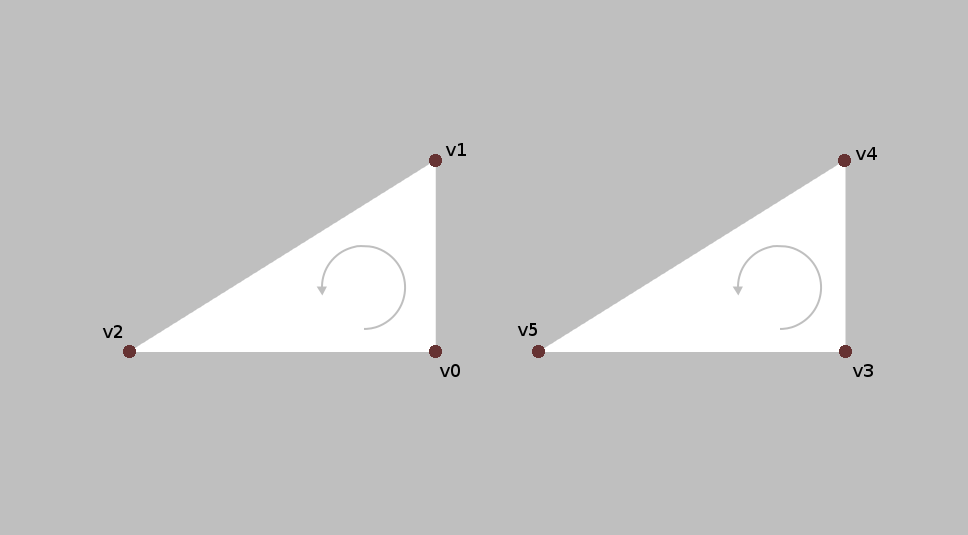
\includegraphics[width=\columnwidth]{culling1.png}
\caption{Non-culled triangles.}
\label{fig:nonculled}
\end{figure}
However, if we flip the \textit{orientation} for the left triangle by using the indices $\{0, 2, 1, 3, 4, 5\}$ instead, the triangle dissapears entirely!
\begin{figure}[H]
\centering
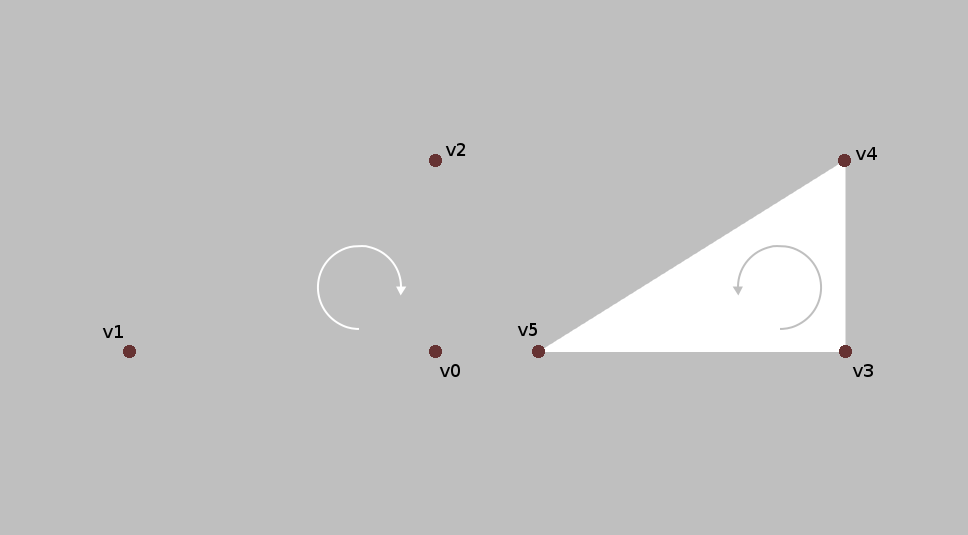
\includegraphics[width=\columnwidth]{culling2.png}
\caption{Left triangle culled, right triangle not.}
\label{fig:nonculled}
\end{figure}
The result we see in figure \ref{fig:nonculled} might seem strange, but it is in fact a very important part of the OpenGL rendering pipeline called \textit{face culling}. The rule OpenGL goes by in the default case is to only render faces (triangles) that are \textit{counter clockwise winding}, like we see here. This rule can be toggled to render the opposite winding by use of the function \texttt{void glFrontFace(GLenum mode);} which takes in either \texttt{GL\_CW} or \texttt{GL\_CCW} for clockwise and counter clockwise winding, respectively.
\subsection{}
\begin{enumerate}
\item The depth buffer is used to determine which parts of a scene should be rendered and which should not due to other objects being in front of them. This test, called a \textit{depth test} is enabled with the function \texttt{glEnable(GL\_DEPTH\_TEST)}. Since this option is enabled, we must clear the depth buffer after each render, or the current frame will use the depth values from the last frame.
\item The fragment shader is executed once \textit{for each fragment}, not each pixel. These concepts, although similar, are not entirely the same. This means that the shader can sometimes be executed more than once for the same pixel. Examples include if we want to make some kind of transparent materials, or try to implement antialiasing in the fragment shader. Say OpenGL is trying to color a pixel that happens to be at the very corner of a yellow triangle that is in turn in front of a red background. The pixel will be colored somewhere in-between yellow and red, instead of one or the other.
\item The two kinds of shaders we use a lot are the \textit{vertex shader} and the \textit{fragment shader}. The vertex shader is one of the first steps in the OpenGL rendering pipeline, and it handles taking the vertices given to it as vertex attribute data and actually generates vertices (transforms and projects them onto the camera) for further processing by the vertex post-processing stage. The fragment shader takes in \textit{rasterized} fragments and colors them. In addition, it sets the depth value of the fragment.
\item By specifying the order the vertices should be drawn in through indices, OpenGL makes it possible to render the same vertex multiple times whithout having to specify it more than once. This is hugely beneficial when rendering more complex objects than a simple triangle, e.g. a cube, where the corner vertices will be part of multiple triangles. Many executions of the vertex shader can be saved for each object like this.
\item The pointer value tells OpenGL where it should start reading the buffer. By passing a non-zero value, we tell it to start reading further into the buffer than from the beginning.
\end{enumerate}
\subsection{}
We begin with the following scene (figure \ref{fig:tris_red_bg}).
\begin{figure}[H]
\centering

\includegraphics[width=\columnwidth]{tris_red_bg.png}
\caption{Two triangles on a red background.}
\label{fig:tris_red_bg}
\end{figure}
The first task is to mirror this scene both horisontally and vertically. This is easily accomplished by flipping the signs on the $x$ and $y$ coordinates of each vertex in the vertex shader. This results in the following mirrored scene (figure \ref{fig:tris_mirrored}).
\begin{figure}[H]
\centering

\includegraphics[width=\columnwidth]{mirrored-tris.png}
\caption{Two flipped triangles mirrored both horisontally and vertically.}
\label{fig:tris_mirrored}
\end{figure}
Finally we will change the color of the triangles, and this time we want to try our hands at a gradient. We can obtain the position of each fragment from \texttt{vec4 gl\_FragCoord}, so an easy way to do this would be to make the r, g and b values depend on for instance the $x$ value of the current fragment, which would make a nice grayscale gradient going across the screen. RGB values are however quite unintuitive to work with, so it would be much better to have a hue-based color mapping. A quick google search yields us a GLSL snippet for converting from the HSV color space into RGB. Feeding in the $x$ coordinate into the hue while leaving the saturation and value both at 1 produces the slick triangles in figure \ref{fig:tris_wavy}.
\begin{figure}[H]
\centering
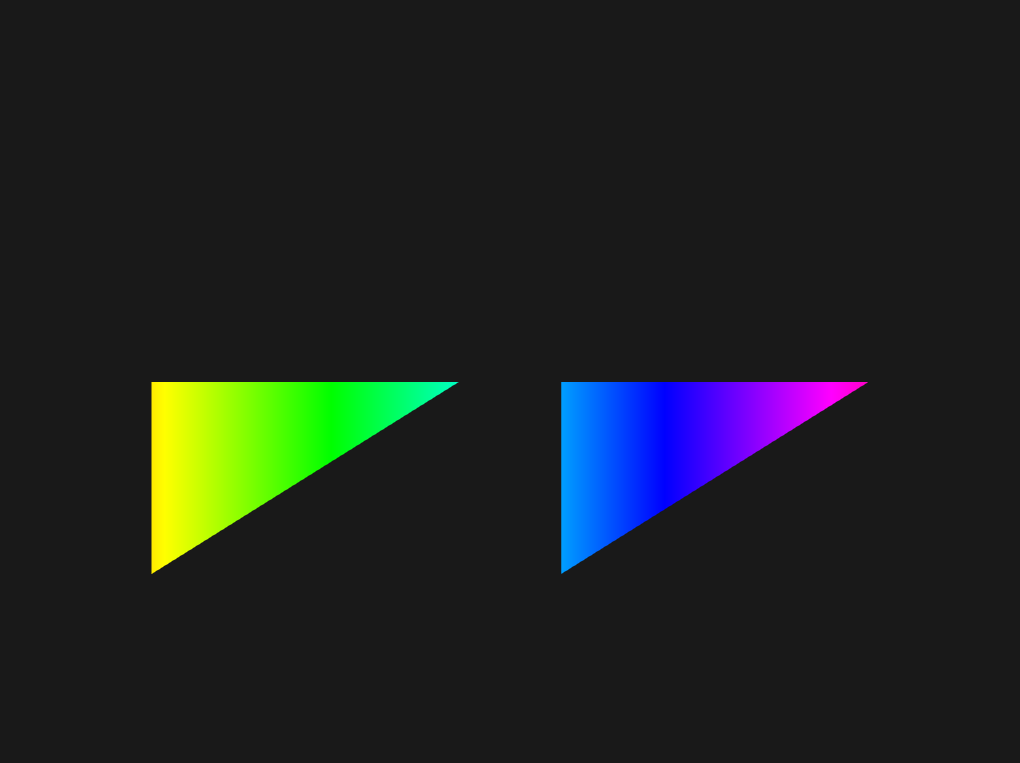
\includegraphics[width=\columnwidth]{mirrored_color_tris.png}
\caption{Two gradient-colored triangles.}
\label{fig:tris_wavy}
\end{figure}

\section{Bonus!}
\subsection{Checkerboard}
Drawing a checkerboard can be done by dividing the $x$ coordinate with some length (that will be the size of our checker squares) and then taking the modulus with $2$. This first result in a zebra pattern. If we do the same calculation with the $y$ coordinate as well and compute the exclusive OR with the x-one, we get the checker pattern we are after. See figure \ref{fig:tris_checker}.
\begin{figure}[H]
\centering
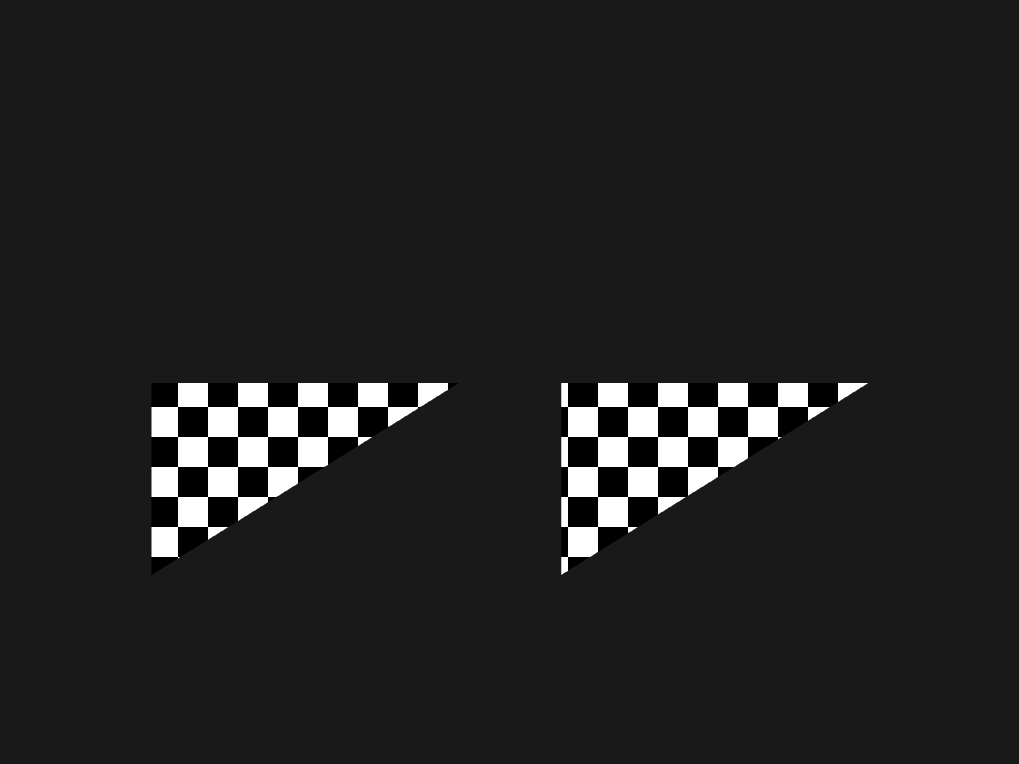
\includegraphics[width=\columnwidth]{checker.png}
\caption{Checkerboard triangles.}
\label{fig:tris_checker}
\end{figure}

\subsection{Circle and sine function}
We define a function to take in a vector of $x$ coordinates and a function, and output a vector corresponding of $y$ coordinates. This can in turn be used to create a circle, by using the functions
\begin{equation}\begin{aligned}
f_{\text{U}}(x) = \sqrt{r^2 - x^2},  \quad f_{\text{L}}(x) = -\sqrt{r^2 - x^2}
\end{aligned}\end{equation}
as input, or a sine by using a \texttt{std::sin} as input. For the circle, we render it using \texttt{GL\_TRIANGLE\_FAN}, making sure to orient the upper and lower half-circle according to the face-culling rule we have chosen. This results in the render in figure \ref{fig:circle} below.
\begin{figure}[H]
\centering

\includegraphics[width=\columnwidth]{circle.png}
\caption{Circle}
\label{fig:circle}
\end{figure}
For the sine (this is really task \textbf{e}), we use \texttt{GL\_LINE\_STRIP} to produce the render in figure \ref{fig:sine} below.
\begin{figure}[H]
\centering
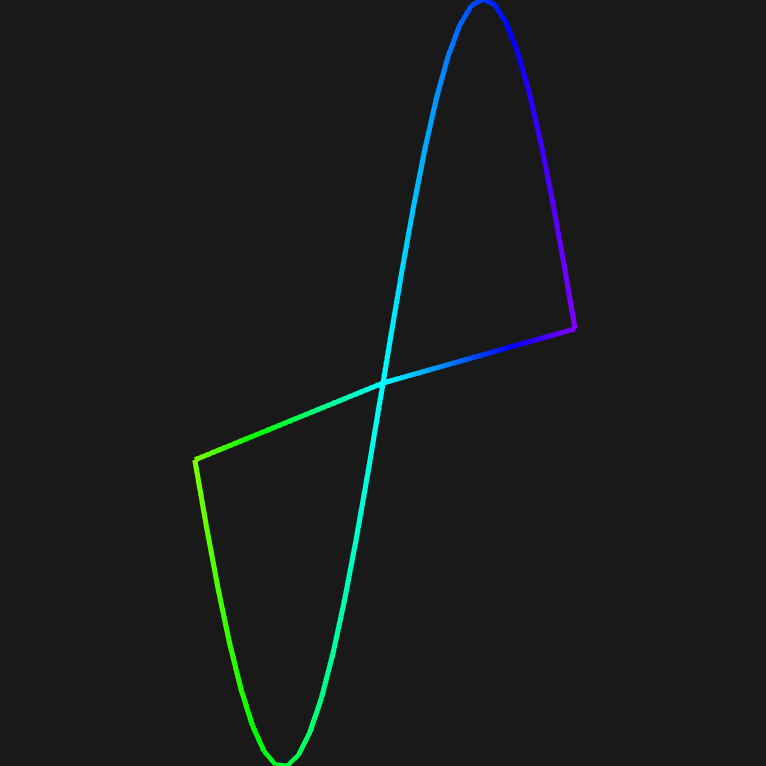
\includegraphics[width=\columnwidth]{sine.png}
\caption{Sine function.}
\label{fig:sine}
\end{figure}
Notice how OpenGL draws a rogue line that is not really part of the sine function.


\end{multicols}

\end{document}

